\section{Pilot system}
\label{sec:pilot-study:pilot-system}

The pilot system high-level architecture, as shown in Figure
~\ref{fig:pilot-study:pilot-system:architecture}, is comprised of
three sub-layers: the client sub-layer, described in Section
~\ref{sec:pilot-study:pilot-system:user-interface}, provides an entry point
through with end user interact with the system; the service sub-layer is
composed of services through which end users interact with digital objects; and
the repository sub-layer, described in Section
~\ref{sec:pilot-study:pilot-system:repository},  provides storage
structures for the digital objects.

\subsection{User interface}
\label{sec:pilot-study:pilot-system:user-interface}

\begin{figure}
 \centering
 \framebox[\textwidth]{
 % Generated with LaTeXDraw 2.0.8
% Sun Sep 23 01:32:25 SAST 2012
% \usepackage[usenames,dvipsnames]{pstricks}
% \usepackage{epsfig}
% \usepackage{pst-grad} % For gradients
% \usepackage{pst-plot} % For axes
\scalebox{1} % Change this value to rescale the drawing.
{
\begin{pspicture}(0,-3.6)(9.092343,3.6)
\definecolor{color55}{rgb}{0.9372549019607843,0.1450980392156863,0.10588235294117647}
\definecolor{color2146}{rgb}{0.9529411764705882,0.08627450980392157,0.054901960784313725}
\psframe[linewidth=0.04,dimen=outer](8.862344,3.6)(0.8623437,2.4)
\psline[linewidth=0.06cm,linestyle=dashed,dash=0.16cm 0.16cm](0.66234374,2.0)(9.062344,2.0)
\psframe[linewidth=0.04,dimen=outer](8.862344,1.58)(0.8623437,-0.02)
\psframe[linewidth=0.03,dimen=outer](3.4623437,1.1)(1.4623437,0.5)
\psframe[linewidth=0.03,dimen=outer](5.862344,1.1)(3.8623438,0.5)
\psframe[linewidth=0.03,dimen=outer](8.262343,1.1)(6.262344,0.5)
\psline[linewidth=0.06cm,linestyle=dashed,dash=0.16cm 0.16cm](0.66234374,-0.5)(9.062344,-0.5)
\usefont{T1}{ppl}{m}{n}
\rput(4.8028126,2.995){\footnotesize Web Browser}
\usefont{T1}{ppl}{m}{n}
\rput(2.3795311,0.795){\footnotesize Search}
\usefont{T1}{ppl}{m}{n}
\rput(4.7965627,0.795){\footnotesize Browse}
\usefont{T1}{ppl}{m}{n}
\rput(7.276094,0.795){\footnotesize Index}
\psframe[linewidth=0.04,dimen=outer](8.862344,-1.0)(0.8623437,-3.6)
\psframe[linewidth=0.03,dimen=outer](5.6223435,-2.38)(3.6223438,-2.98)
\psframe[linewidth=0.03,dimen=outer](3.4423437,-2.4)(1.4423437,-2.98)
\usefont{T1}{ppl}{m}{n}
\rput(4.6021876,-2.705){\footnotesize Images}
\usefont{T1}{ppl}{m}{n}
\rput(2.4301562,-2.705){\footnotesize Metadata}
\usefont{T1}{ppl}{m}{n}
\rput{-270.0}(3.1914062,2.7823439){\rput(0.18546875,2.96){\small Client}}
\usefont{T1}{ppl}{m}{n}
\rput{-270.0}(0.9907812,0.66296875){\rput(0.14140625,0.8){\small Services}}
\usefont{T1}{ppl}{m}{n}
\rput{-270.0}(-2.1415625,-2.470625){\rput(0.13109376,-2.3){\small Repository}}
\psframe[linewidth=0.03,dimen=outer](8.442344,-1.8)(6.4423437,-2.4)
\usefont{T1}{ppl}{m}{n}
\rput(7.3948436,-2.085){\footnotesize HTML}
\usefont{T1}{ppl}{m}{n}
\rput(4.768906,-1.465){\footnotesize File System}
\psframe[linewidth=0.06,linecolor=color55,linestyle=dashed,dash=0.16cm 0.16cm,dimen=outer](5.842344,-2.02)(1.2423438,-3.36)
\psframe[linewidth=0.03,dimen=outer](8.442344,-2.62)(6.4423437,-3.2)
\usefont{T1}{ppl}{m}{n}
\rput(7.4521875,-2.925){\footnotesize Indicies}
\psframe[linewidth=0.06,linecolor=color2146,linestyle=dashed,dash=0.16cm 0.16cm,dimen=outer](8.622344,-1.54)(6.222344,-3.38)
\end{pspicture} 
}


 }
 \caption{Pilot system architecture}
 \label{fig:pilot-study:pilot-system:architecture}
\end{figure}

The pilot implementation has one publicly-accessible user interface, accessible
via a standard Web browser, that end users use to interact with the
digital objects. Figure ~\ref{fig:pilot-study:pilot-system:user-interface} is
a screenshot of the pilot system user interface, rendered in a Web browser. The
interaction with digital objects is implicitly done through two standard
services --search and browse.

\begin{figure}
 \centering
 \framebox[\textwidth]{%
 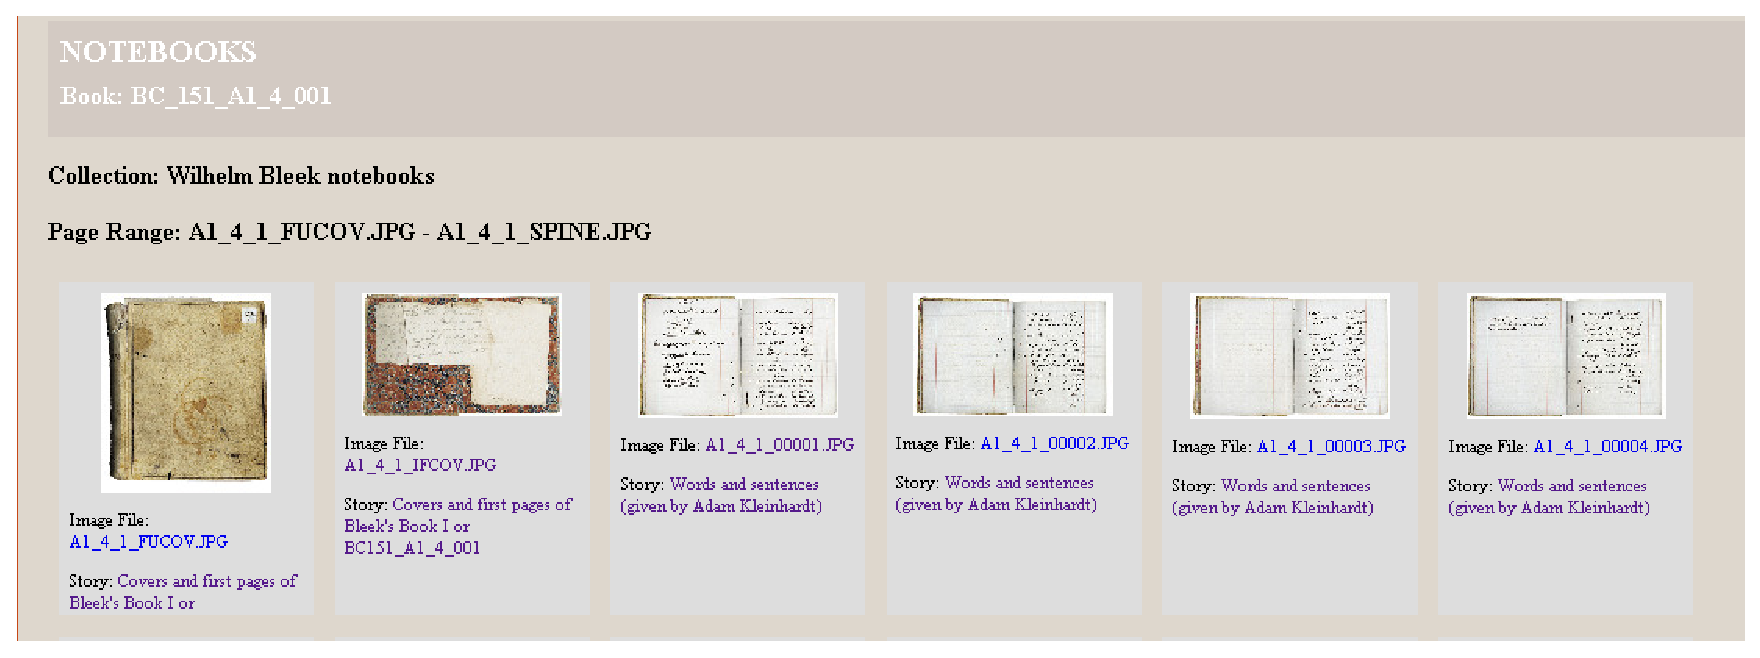
\includegraphics[width=0.95\textwidth]{%
 chapter03/figures/pilot-implementation-screenshot.eps}
 }%
 \caption{Pilot system user interface}
 \label{fig:pilot-study:pilot-system:user-interface}
\end{figure}

The user interface is rendered using statically-generated HTML files, that are
generated by applying XSLT stylesheets to individual metadata objects. The
metadata object structure is discussed in detail in Section
~\ref{sec:pilot-study:pilot-system:repository}

\subsection{Repository}
\label{sec:pilot-study:pilot-system:repository}

The repository sub-layer stores both the digital content and associated
representational information --metadata objects-- on the filesystem, alongside
each other, with the metadata objects stored in XML plain text files. The
digital objects are contained within hierarchical folders, hereon called
containers objects, that conform to the original original collection structure. 

The metadata file records were encoded using a qualified dublin application
profile \citep{Coyle2009} that was created specifically for the Bleek and Lloyd
collection, with each object having one associated metadata file. Three
distinct types of metadata objects were devised: container metadata objects,
illustrated in Listing ~\ref{lst:pilot-study:pilot-system:container}, are
essentially manifests of digital objects contained within them; virtual
objects, illustrated in Listing ~\ref{lst:pilot-study:pilot-system:virtual},
define the semantics of the images and collection as a whole by describing the
logical association of the images and collection; and digital content metadata
objects encode representational information specific to each individual image.

\lstinputlisting[float,frame=lines,caption=A digital content metadata file, label=lst:pilot-study:pilot-system:content, language=XML]{chapter03/code/digital-content.metadata}

\lstinputlisting[float,frame=lines, caption=A virtual object metadata file, label=lst:pilot-study:pilot-system:virtual,language=XML]{chapter03/code/virtual-object.metadata}

\lstinputlisting[float,frame=lines,caption=A container object metadata file,label=lst:pilot-study:pilot-system:container,language=XML]{ chapter03/code/container-object.metadata }